\begin{frame}
    \frametitle{Generalization}
    \vspace*{0.8cm}
Motivation: Key question in deep learning: How well does my NN perform on unseen data?


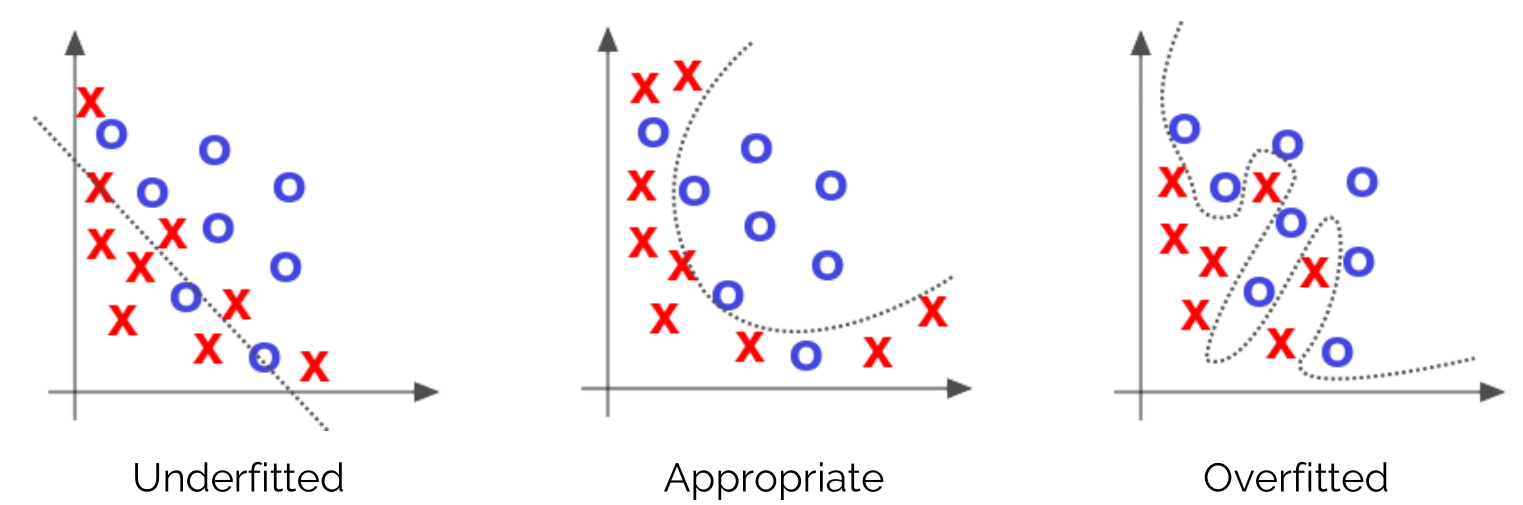
\includegraphics[width=0.85\textwidth, height=.5\textheight]{./Ressourcen/Praesentation/Bilder/generalization.png}%

\vspace*{-0.6cm}

Taken from Deep Learning by Adam Gibson, Josh Patterson, O'Reily Media Inc., 2017

\end{frame}
\clearpage

\begin{frame}
    \frametitle{Generalization}
    \vspace*{0.8cm}
To test generalization new datasets need to be created

Generation of $1$ training sample:  $\approx 70$ seconds (using Google Colab)

Generation of $12.8k$ training samples: $> 10$ days -- not feasible 

$\implies$ Generate only new test sets containing $90$ samples: $< 2$ hours -- feasible

Extrapolation with different angle of attack intervals, default: $[-22.5, 22.5]$:

\begin{PraesentationAufzaehlung}
    \item $[-45, 45]$
    \item $[-90, 90]$
    \item $[-67.5, -22.5]$
    \item $[22.5, 67.5]$
\end{PraesentationAufzaehlung}


\end{frame}
\clearpage

%%%%%%%%%%%%%%%%%%%%%%%%%%%%%%%%%%%%%%%%%%%%%%%%%%%%%
%% Folie: Diagramm                                 %%
%%%%%%%%%%%%%%%%%%%%%%%%%%%%%%%%%%%%%%%%%%%%%%%%%%%%%
\begin{frame}
    \frametitle{Generalization -- Evaluation}
Error increase of different angle of attack intervals wrt. ground truth $[-22.5 , 22.5]$
\begin{center}
	\vspace*{-1cm}
    \begin{tikzpicture}
        \begin{axis}[
                ybar=10,
                bar width=27.1,
                axis line style={transparent},
                every tick/.style={transparent},
                enlarge x limits=0.145, % X-Achse skalieren
                clip limits=true,
                ymin=0,
                ymax=30,
                width=\textwidth,
                height=.65\textheight,
                symbolic x coords={-45 -- 45,-90 -- 90,-67.5 -- -22.5,22.5 -- 67.5},
                xticklabels={-45 -- 45,-90 -- 90,-67.5 -- -22.5,22.5 -- 67.5},
                xtick=data,
                ytick={0,5,10,15,20,25},
                every tick label/.append style={font=\fontsize{13}{14}\selectfont},
                ymajorgrids,
                legend image code/.code={\draw[draw=none] (0cm,-0.12cm) rectangle (0.29cm,0.17cm);}, % Legenden-Symbol  
                legend columns=3,
                reverse legend,
                legend style={
                    font={\usebeamerfont{footnote}},
                    fill=none,
                    draw=none,
                    /tikz/every odd column/.append style={column sep=0.07cm}, % Abstand zwischen Legenden-Symbol
                    /tikz/every even column/.append style={column sep=0.8cm} % Abstand zwischen den Legendeneinträgen
                 },
                legend to name=PraesentationDiagrammVertikalLegende
            ]
            
            \addlegendentry{Combined}        
            \addlegendentry{Pressure}    
            \addlegendentry{Velocity}    
            
            \addplot[color=TUMBlauDunkel, fill=TUMBlauDunkel] coordinates {
                (-45 -- 45,6.07)
                (-90 -- 90,18.23)
                (-67.5 -- -22.5,15.11)
                (22.5 -- 67.5,22.99)
            };
            
            \addplot[color=TUMBlauHell, fill=TUMBlauHell] coordinates {
                (-45 -- 45,3.66)
                (-90 -- 90,5.73)
                (-67.5 -- -22.5,6.00)
                (22.5 -- 67.5,10.70)
            };
            
            \addplot[color=TUMBlauMittel, fill=TUMBlauMittel] coordinates {
                (-45 -- 45,5.14)
                (-90 -- 90,19.20)
                (-67.5 -- -22.5,13.84)
                (22.5 -- 67.5,23.25)
            };        
        \end{axis}
    \end{tikzpicture}

    \vspace*{-5mm}
    \ref*{PraesentationDiagrammVertikalLegende}%
\end{center}
\end{frame}
\clearpage